\documentclass[11pt]{article}
\usepackage[margin=1in]{geometry}
\usepackage{graphicx}
\usepackage{booktabs}
\usepackage{float}
\usepackage{hyperref}
\usepackage[numbers]{natbib}
\usepackage{caption}
\usepackage{setspace}
\onehalfspacing
\title{Sweat Chemosignals and Facial Micro-Expressions:\\A Computational Video-Analysis Pipeline and Preliminary Exploratory Evidence}
\author{Yogev Git \and Ofir Goldreich \and Nir Shoham \\ Baruch Ivcher School of Psychology, Reichman University}
\date{Draft prepared June 2026}
\begin{document}
\maketitle
\noindent\textbf{Privacy note.} This draft includes only aggregate statistics and non-identifying plots. It does not include participant frames, face crops, contact sheets, or WhatsApp images.

\section*{Abstract}
Human sweat can contain chemosensory information that influences social perception and action even when people do not explicitly identify the source of the odor. The present work develops a privacy-preserving computational pipeline for testing whether sweat-related chemosignals are accompanied by rapid facial responses and candidate micro-expressions during a filmed odor-discrimination task. The current dataset contains 15 representative videos processed at 100 frames per second, yielding 450,805 frame-level observations, 3,614 automatically detected candidate micro-events, and 114 candidate sniff-like windows. A newly added annotation file includes 38 trial rows across 15 videos, with 30 filled sniff onsets, 30 rows marked ok, 6 pending rows, and 2 excluded rows. For the two-test-tube protocol, trial 1 was coded as placebo/control and trial 2 as sweat, producing 22 mapped trial rows and a primary paired subset of 7 complete videos. The resulting sweat-control analyses are reported as preliminary exploratory evidence rather than as a confirmatory test.

\section{Introduction}
Human body odor is not merely a nuisance variable in social interaction. A growing literature suggests that sweat and other chemosensory cues can carry affective and social information, sometimes influencing perception or behavior without being explicitly recognized by the perceiver. Studies of chemosignal communication, interpersonal distance, and affective processing converge on the idea that olfactory cues may shape approach, avoidance, arousal, and evaluative response through pathways that are closely linked to limbic and embodied social systems.

The present project extends that rationale from overt interpersonal behavior to the face itself. In the two-test-tube paradigm, filmed participants smell two coded tubes, one intended to contain human sweat collected in a separate exercise-based sweat-donation study and one serving as a control stimulus. The scientific question is whether the facial response contains an implicit temporal signature of sweat exposure, even when a participant's declarative identification of the tube is inaccurate or incomplete.

Micro-expressions and brief facial movements are theoretically relevant because they may reveal rapid affective or evaluative processing before the participant can regulate or verbalize the response. The Facial Action Coding System decomposes facial behavior into action units, and automated facial-analysis tools make it possible to summarize movement patterns over time. For odor exposure, the nose, upper lip, mouth, and cheek regions are especially important: AU9 and AU10 are associated with nose wrinkling and upper-lip raising, AU6 and AU12 capture cheek and lip-corner movement, and AU45 offers a blink-related marker that can change with sensory sampling or discomfort.

This article therefore describes both the planned experimental logic and the implemented computational video-analysis pipeline. It deliberately separates the methodological achievement of extracting high-frequency facial features from the still-unfinished experimental inference about sweat versus control. That separation is essential: condition should never be inferred from file names or visual inspection. In the present revision, order is used only where the two-test-tube protocol was explicitly clarified: the first tube was placebo/control and the second tube was sweat.

\section{Research Questions and Hypotheses}
The primary research question is whether dynamic facial-expression measures differ after sniffing a sweat tube compared with a control tube. A second question asks whether this difference can be observed even when explicit tube identification is incorrect, which would support a partial or implicit chemosensory response. A third question concerns which measures and time windows are most informative, with a particular emphasis on cheek, nose, upper-lip, blink, and mouth-related proxies.

The working hypotheses are directional but remain exploratory in the current version. Sweat trials are expected to show faster or stronger changes in measures linked to aversion, alertness, cautious sampling, or facial tension. Early windows after sniff onset are expected to be more sensitive to micro-expression-like responses than later windows, whereas later windows may include more deliberate expression regulation. The cheek composite is treated as a preregistered analytic priority because it summarizes AU6/AU12-related movement and adjacent geometric change.

\section{Method}
The project distinguishes two samples. Sweat donors are the individuals from whom sweat samples were collected in a separate spinning-exercise study. Filmed participants are a separate group who complete the odor-exposure task. This distinction matters ethically and analytically: the person providing the sweat sample is not the person whose face is analyzed in the video.

The target design is within-subjects. Each filmed participant smells coded tubes, and the central independent variable is stimulus type: sweat versus control. The principal dependent variables are facial-expression proxies, candidate micro-events, latency to response, peak response, area under the curve, explicit identification accuracy, and trial-level quality measures. For the two-test-tube protocol analyzed here, the first tube was coded as placebo/control and the second tube was coded as sweat. This rule was not applied to four-trial odor sequences.

The current video inventory contains 19 MP4 files. Four exact duplicates were identified and excluded from representative counts, leaving 15 representative videos for automatic analysis. The annotations contain 11 two-test-tube videos and 4 four-trial odor-sequence videos. The two-test-tube videos define the sweat/control analysis set; four-trial rows are retained for traceability and exploratory timing work but are not merged into the sweat/control hypothesis test.

\section{Computational Video-Analysis Pipeline}
The implemented pipeline reads source videos in place, leaving the original recordings unchanged. It uses OpenCV for video access, MediaPipe-derived facial landmarks for geometry-based measurement, and DeepFace as a low-frequency auxiliary emotion layer. DeepFace is not treated as a substitute for FACS or for micro-expression measurement; it is used only as an additional descriptive layer.

The full representative dataset was processed at 100 frames per second. For each frame, the system extracted geometry-based proxies for cheek raising, lip-corner movement, nose wrinkling, upper-lip raising, lip press or mouth opening, blinking, asymmetry, and head movement. The pipeline then summarized short-lived deviations from a rolling baseline as candidate micro-events when they exceeded a robust z-score threshold and lasted within the target micro-event duration range.

The current extraction produced 450,805 processed frame rows across 15 representative videos. DeepFace sample files were present for 15 videos. The automatic detector found 3,614 candidate micro-events; the most frequent metrics were AU45 blink=643, AU6 cheek raise=423, AU9 nose wrinkle=415, cheek composite=378, AU10 upper-lip raise=324, AU24 lip press=302. The median event duration was 0.150 s and the median peak absolute robust z-score was 4.14.

\section{Annotation and Quality Control}
Manual annotation remains the key step separating exploratory feature extraction from confirmatory experimental inference. The current annotations file contains 38 rows across 15 videos. Sniff onset is filled in 30 rows; approach onset and response time are not yet filled in the current annotations file. The quality flags are ok=30, pending=6, and exclude=2.

The condition mapping now contains 22 rows from the two-test-tube protocol. The primary paired analysis uses 7 complete videos (14 trial rows) in which both trials were marked ok and had a sniff onset. 8 two-test-tube rows remain pending or excluded and were not included in the paired comparison.

Quality control was computed at the video level. The mean face-detection rate was 0.939. The quality tiers were good=13, usable\_review=1, and review\_or\_exclude=1. The lower-quality videos should be reviewed manually before any final group-level inference.

The analysis uses strict privacy boundaries. The article includes only aggregate plots and numeric summaries. It does not include participant frames, face crops, contact sheets, WhatsApp images, or other potentially identifying visual material.

\section{Preliminary Exploratory Results}
The current results show that the computational layer is operational across the full representative dataset. The system successfully generated frame-level features, video-level quality summaries, candidate micro-events, candidate sniff-like windows, correlation plots, and exploratory PCA/clustering summaries. These results are best understood as a feasibility and data-readiness outcome.

The automatic sniff-window detector identified 114 candidate sniff-like windows. These windows are useful for prioritizing human review, but they are not final event labels. The trial-level paired report generated 132 sweat-control comparison rows across baseline-normalized AU-proxy summaries. These comparisons use n=7 paired videos and should be interpreted as preliminary because the sample is small and the facial measures are automated proxies. The lowest-p preliminary rows were late\_2\_5s / cheek composite: mean sweat-control difference=-0.0365, dz=-1.4, paired t p=0.009; early\_0\_500ms / head roll deg: mean sweat-control difference=5.23, dz=0.94, paired t p=0.0474; short\_500\_2000ms / head roll deg: mean sweat-control difference=5.17, dz=0.82, paired t p=0.0725.

The non-identifying figures included with this draft visualize the quality distribution, event density, event-duration distribution, correlations among facial metrics, and unsupervised PCA and clustering structure. They support pipeline validation and exploratory profiling. The condition-level tables add a first paired sweat/control layer, but they do not by themselves establish a final condition-specific chemosignal effect.

\begin{table}[H]
\centering
\caption{Current data-readiness summary.}
\begin{tabular}{ll}
\toprule
Item & Current value \\
\midrule
Representative videos processed & 15/15 \\
Processed frame rows & 450,805 \\
Candidate micro-events & 3,614 \\
Candidate sniff-like windows & 114 \\
Annotation rows & 38 \\
Filled sniff onsets & 30 \\
Two-test-tube condition mapping rows & 22 \\
Primary paired videos & 7 \\
Paired sweat/control comparison rows & 132 \\
\bottomrule
\end{tabular}
\end{table}

\begin{figure}[H]
\centering
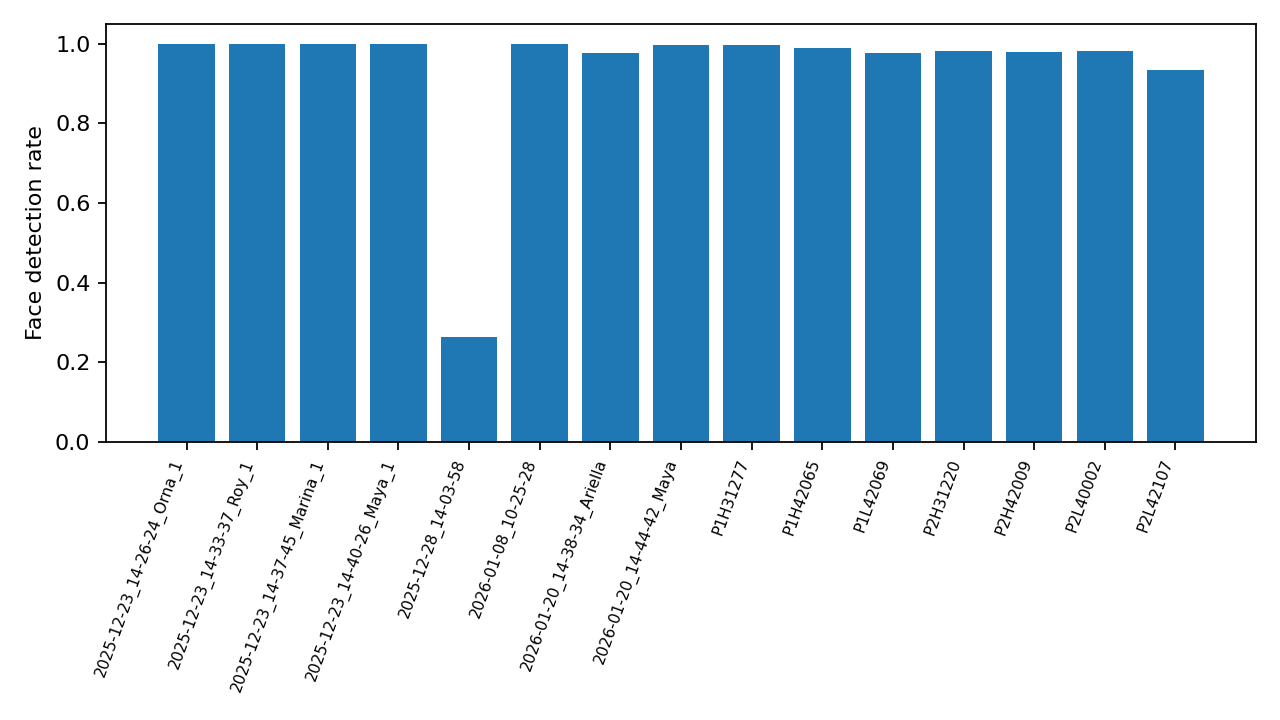
\includegraphics[width=0.92\linewidth]{figures/quality_face_detection_rate.png}
\caption{Video-level face-detection quality across the representative dataset.}
\label{fig:quality}
\end{figure}

\begin{figure}[H]
\centering
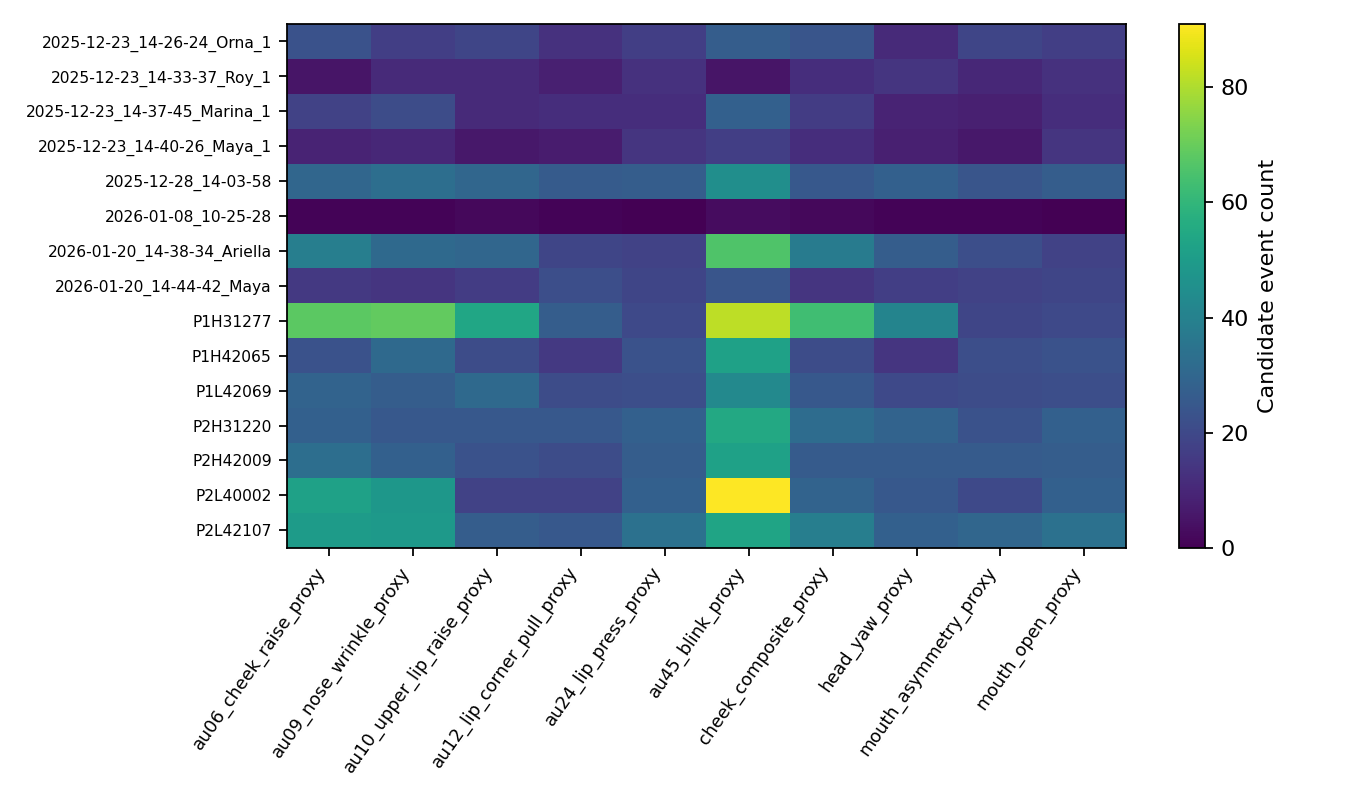
\includegraphics[width=0.92\linewidth]{figures/event_count_heatmap.png}
\caption{Candidate micro-event density by video and metric.}
\label{fig:event-heatmap}
\end{figure}

\begin{figure}[H]
\centering
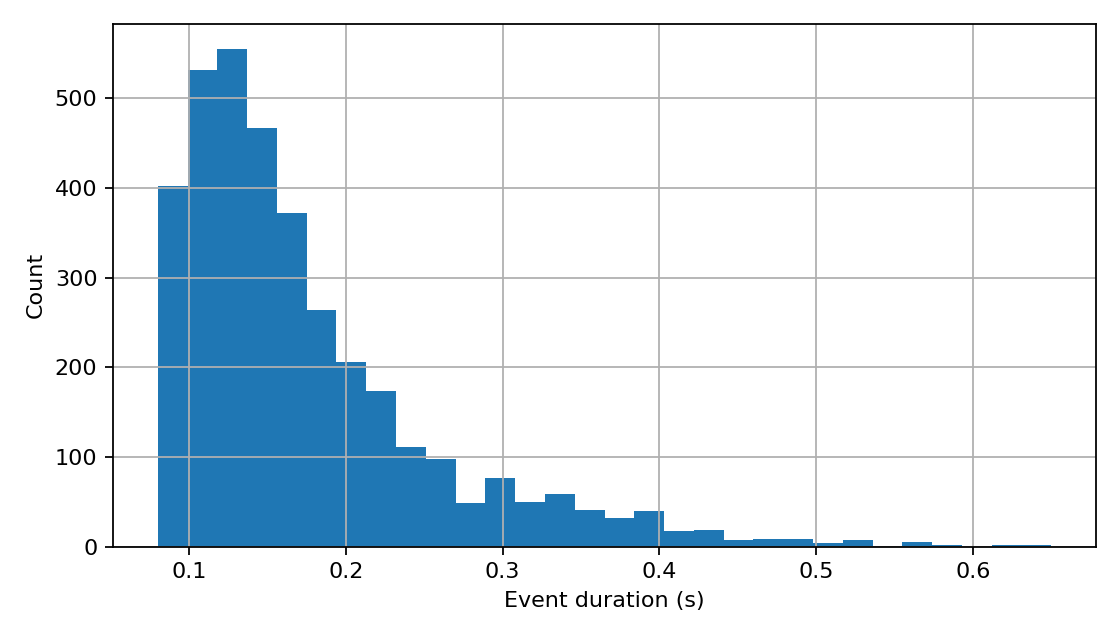
\includegraphics[width=0.92\linewidth]{figures/event_duration_histogram.png}
\caption{Distribution of automatically detected candidate event durations.}
\label{fig:event-duration}
\end{figure}

\begin{figure}[H]
\centering
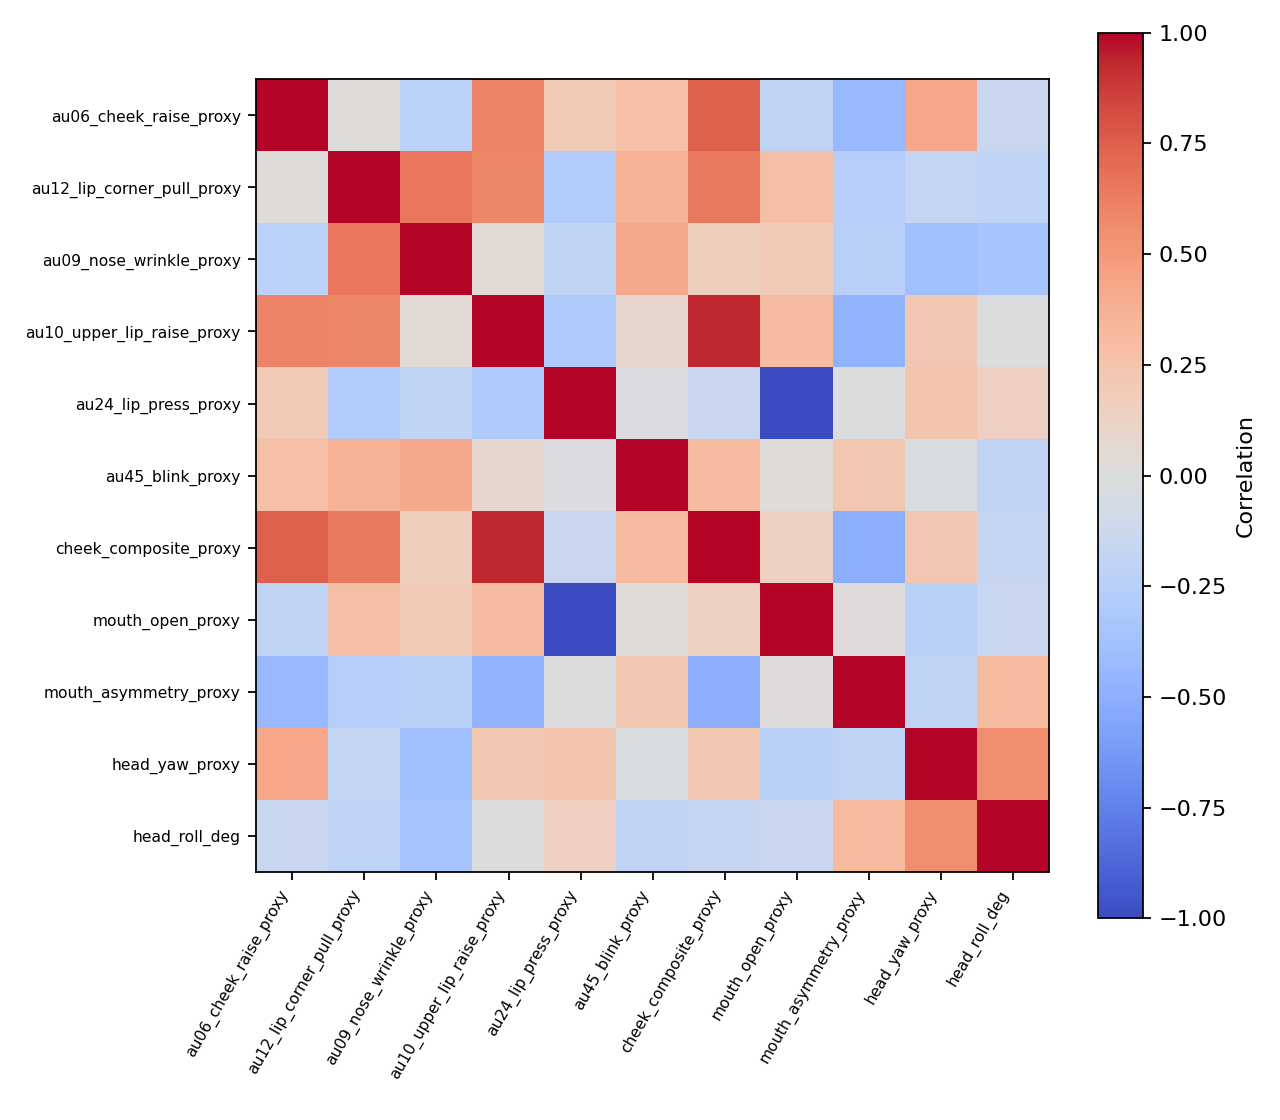
\includegraphics[width=0.92\linewidth]{figures/metric_correlation_heatmap.png}
\caption{Correlations among video-level facial metric summaries.}
\label{fig:correlations}
\end{figure}

\begin{figure}[H]
\centering
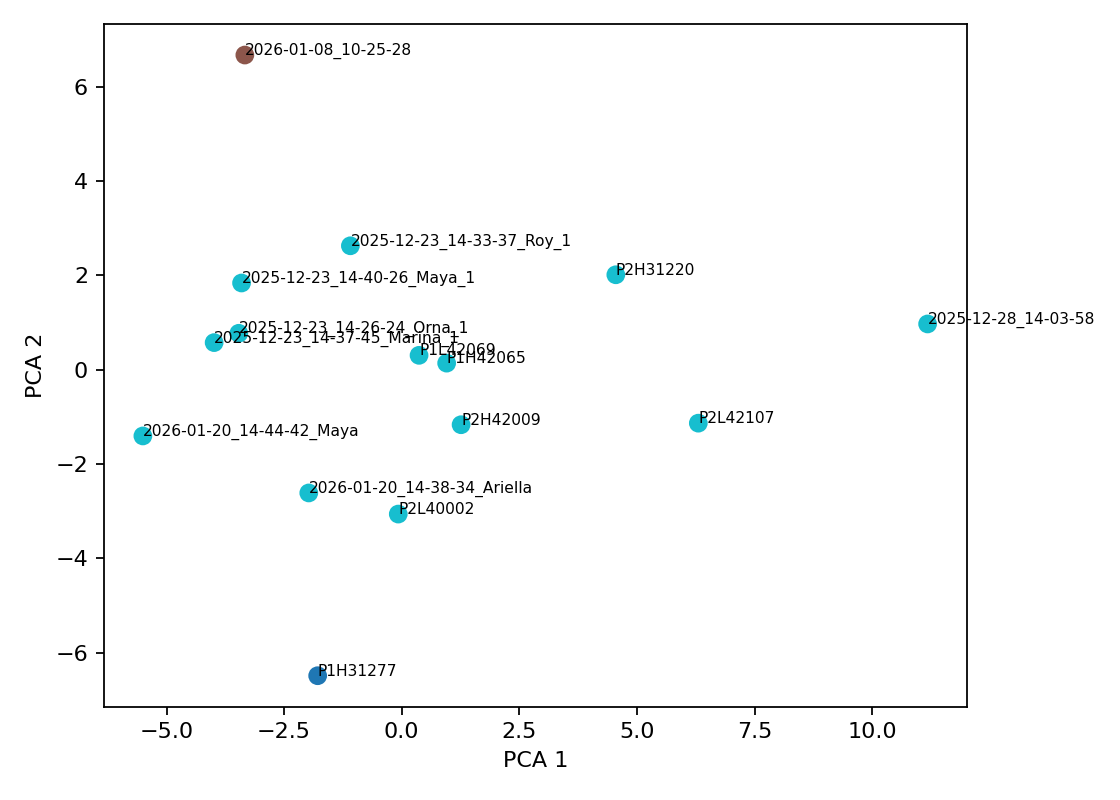
\includegraphics[width=0.92\linewidth]{figures/pca_cluster_plot.png}
\caption{Exploratory PCA and clustering profile across representative videos.}
\label{fig:pca}
\end{figure}

\section{Discussion}
The main contribution of the present work is a reproducible bridge between a psychologically motivated chemosignal question and a high-frequency computational facial-analysis workflow. The pipeline turns raw video into interpretable numeric summaries while preserving participant privacy and making uncertainty visible through explicit quality-control fields.

The project is now positioned for a stronger next analysis step. The two-test-tube subset already has a protocol-based sweat/control mapping, allowing paired tests and Wilcoxon signed-rank tests on baseline-normalized trial summaries. As more timings and condition metadata are completed, permutation tests and mixed-effects models will be appropriate for testing robustness and handling participant-level variability.

The current annotation file also clarifies an important design issue. Some rows appear to reflect a four-trial odor protocol rather than the planned two-test-tube sweat/control paradigm. Rather than forcing these data into the main model, the article treats them as a separate protocol category requiring supervisor clarification. This conservative handling protects the validity of any later inference.

\section{Limitations and Next Steps}
The central limitation is no longer the absence of condition labels for the two-test-tube subset, but the limited size and completeness of the analyzable paired sample. The current primary condition analysis is based on 7 complete paired videos, while pending/excluded two-test-tube rows and all four-trial rows remain outside the main sweat/control test. A second limitation is that automatic facial geometry proxies are not FACS-certified AU labels; they should be treated as measurable approximations that require careful interpretation and, ideally, human-coded validation on a subset.

Immediate next steps are to confirm the remaining pending sniff onsets, decide whether the four-trial odor protocol has its own condition mapping, and review the videos flagged by quality control. After manual review, the trial-level extraction and analysis commands should be rerun so that paired statistical tests and model-ready tables are based on validated experimental inputs.

\nocite{*}
\bibliographystyle{plainnat}
\bibliography{references}
\end{document}